%%%%%%%%%%%%%%%%%%%%%%%%%%%%%%%%%%%%%%%%%
% Arsclassica Article
% LaTeX Template
% Version 1.1 (1/8/17)
%
% This template has been downloaded from:
% http://www.LaTeXTemplates.com
%
% Original author:
% Lorenzo Pantieri (http://www.lorenzopantieri.net) with extensive modifications by:
% Vel (vel@latextemplates.com)
%
% License:
% CC BY-NC-SA 3.0 (http://creativecommons.org/licenses/by-nc-sa/3.0/)
%
%%%%%%%%%%%%%%%%%%%%%%%%%%%%%%%%%%%%%%%%%

%----------------------------------------------------------------------------------------
%	PACKAGES AND OTHER DOCUMENT CONFIGURATIONS
%----------------------------------------------------------------------------------------

\documentclass[
12pt, % Main document font size
a4paper, % Paper type, use 'letterpaper' for US Letter paper
oneside, % One page layout (no page indentation)
%twoside, % Two page layout (page indentation for binding and different headers)
headinclude,footinclude, % Extra spacing for the header and footer
BCOR5mm, % Binding correction
]{scrartcl}
\usepackage[english]{babel}
\usepackage{url}
\usepackage{graphicx}
\usepackage{subcaption}
\usepackage{float}
\usepackage{epigraph}
\usepackage{mathcomp}
\usepackage{textcomp}
\usepackage{amsmath}
\usepackage{url}

%%%%%%%%%%%%%%%%%%%%%%%%%%%%%%%%%%%%%%%%%
% Arsclassica Article
% Structure Specification File
%
% This file has been downloaded from:
% http://www.LaTeXTemplates.com
%
% Original author:
% Lorenzo Pantieri (http://www.lorenzopantieri.net) with extensive modifications by:
% Vel (vel@latextemplates.com)
%
% License:
% CC BY-NC-SA 3.0 (http://creativecommons.org/licenses/by-nc-sa/3.0/)
%
%%%%%%%%%%%%%%%%%%%%%%%%%%%%%%%%%%%%%%%%%

%----------------------------------------------------------------------------------------
%	REQUIRED PACKAGES
%----------------------------------------------------------------------------------------

\usepackage[
nochapters, % Turn off chapters since this is an article        
beramono, % Use the Bera Mono font for monospaced text (\texttt)
eulermath,% Use the Euler font for mathematics
pdfspacing, % Makes use of pdftex’ letter spacing capabilities via the microtype package
dottedtoc % Dotted lines leading to the page numbers in the table of contents
]{classicthesis} % The layout is based on the Classic Thesis style

\usepackage{arsclassica} % Modifies the Classic Thesis package

\usepackage[T1]{fontenc} % Use 8-bit encoding that has 256 glyphs

\usepackage[utf8]{inputenc} % Required for including letters with accents

\usepackage{graphicx} % Required for including images
\graphicspath{{Figures/}} % Set the default folder for images
 % Include the structure.tex file which specified the document structure and layout
\sloppy
\hyphenation{Fortran hy-phen-ation} % Specify custom hyphenation points in words with dashes where you would like hyphenation to occur, or alternatively, don't put any dashes in a word to stop hyphenation altogether

%----------------------------------------------------------------------------------------
%	TITLE AND AUTHOR(S)
%----------------------------------------------------------------------------------------

\title{\normalfont{A statistical analysis on factors that contributed/slowed down the spread of COVID-19}} % The article title

\subtitle{Project for the exam: Machine learning, statistical learning, deep learning and artificial intelligence} % Uncomment to display a subtitle


\author{Marzio De Corato} % The article author(s) - author affiliations need to be specified in the AUTHOR AFFILIATIONS block

\date{\today} % An optional date to appear under the author(s)

%----------------------------------------------------------------------------------------

\begin{document}



%----------------------------------------------------------------------------------------
%	HEADERS
%----------------------------------------------------------------------------------------

\renewcommand{\sectionmark}[1]{\markright{\spacedlowsmallcaps{#1}}} % The header for all pages (oneside) or for even pages (twoside)
%\renewcommand{\subsectionmark}[1]{\markright{\thesubsection~#1}} % Uncomment when using the twoside option - this modifies the header on odd pages
\lehead{\mbox{\llap{\small\thepage\kern1em\color{halfgray} \vline}\color{halfgray}\hspace{0.5em}\rightmark\hfil}} % The header style

\pagestyle{scrheadings} % Enable the headers specified in this block

%----------------------------------------------------------------------------------------
%	TABLE OF CONTENTS & LISTS OF FIGURES AND TABLES
%----------------------------------------------------------------------------------------

\maketitle % Print the title/author/date block

\newpage

\epigraph{ "Text" }

\newpage
\nocite{*}
\setcounter{tocdepth}{2} % Set the depth of the table of contents to show sections and subsections only

\tableofcontents % Print the table of contents

\listoffigures % Print the list of figures

%\listoftables % Print the list of tables

%----------------------------------------------------------------------------------------
%	ABSTRACT
%----------------------------------------------------------------------------------------

\section*{Abstract} % This section will not appear in the table of contents due to the star (\section*)


%----------------------------------------------------------------------------------------
%	AUTHOR AFFILIATIONS
%----------------------------------------------------------------------------------------

%\let\thefootnote\relax\footnotetext{* \textit{Department of Biology, University of Examples, London, United Kingdom}}

%\let\thefootnote\relax\footnotetext{\textsuperscript{1} \textit{Department of Chemistry, University of Examples, London, United Kingdom}}

%----------------------------------------------------------------------------------------

\newpage % Start the article content on the second page, remove this if you have a longer abstract that goes onto the second page


\section{Introduction} \label{introduction}
The recent pandemic diffusion of the virus \textit{SARS-CoV-2} connected to the \textit{COronaVIrus Disease 19} raised up a scientific issue about the different spread ratio among the different population clusters such as cities,regions and states. This behaviour can be ascribed to the fact that the features of these clusters, such as the densities, the public transports as well as the individual mean incomes are very heterogeneous \cite{sebhatu2020explaining,skorka2020macroecology}. Furthermore the individual policies undertaken by the decision maker of these clusters have a large effect on the spread of the virus \cite{block2020social}. A good tool for an analysis about the correlations of the spread of the virus with the cluster feature is the Principal Component Analysis (PCA): this approach allows to visualize in to a single 2D plot the main statistical correlation of a data set. It is worth nothing that this type of analysis represent only the first step for the identification of causal correlation between the features: the findings obtained via PCA should be validated with a model; however this second step is out from the aim of this work. In this work three different type of cluster were considered: the Italian provinces (\textit{province}), the Italian regions (\textit{regioni}), and 150 countries. The choice of the of Italian provinces was motivated by the fact that this the smallest cluster for which the daily cases of COVID19 are easily available, on the other hand the regions provide aggregate data (in particular about the sanitary system) that are not easily retrievable for the provinces. Finally the inclusion of the states is aimed to see if the statistical correlation obtained for the smaller cluster were still valid in a macroscopic scale. For this last cluster the lock-down policy and its effect was not considered, because the data collection of the policies for each 150 countries was too time consuming, however this analysis may be an outlook for a future update of this work. 

\section{Data description} \label{Data_description}
In this section a brief overview about the data analysed is provided: in particular, for each cluster,a brief description is provided  about the data gathering and assembling. 

\subsection{Provinces}
For this cluster the cumulative number of cases of COVID19 up to 24/08/2020 was obtained from the github website of \textit{Protezione Civile} \cite{github-protezionecivile}. The overall number of total cases was than divided (normalized) by the population number of its province. The population number (2019) was retrieved from Istituto Nazionale di Statistica (ISTAT) \cite{ISTAT}. The size of the province was also considered in order to evaluate the density. Since the diffusion of a virus is causally correlated to connectivity and public mobility services \cite{lloyd2001viruses,kraemer2020effect} we considered also a set of economic indices in order to evaluate the industrialization and the wealth of each province: these are the mean income for person (2019), the public transport (2012 measured as demand for resident), the private transport (2012 measured as cars for resident), the pollution and the unemployment ( 2019). The first one was taken from \textit{Ministero dell'Economia e delle Finanze} as reported in the following website \cite{MEF} while the other ones were obtained from the ISTAT databases \cite{ISTAT}.

\subsection{Regions}
As for the provinces also for this cluster the cumulative number of cases of COVID19 was taken from from \cite{github-protezionecivile} up to 24/08/2020. In this case the same source provides the overall number of tests. The unemployment rate as well the mean income were also available from ISTAT \cite{ISTAT} (2019). Since the Italian constitution delegates partially the management of health services to the regions, new features connected to the latter are available. Here we considered the following ones: the number of resident citizens for general practitioner (\textit{medico di base}, the normalized number of structures for hospitalization, the normalized number of medical guards (\textit{guardie mediche}) multiplied by $10^{5}$ and their normalized number of visit performed multiplied by $10^{5}$. These data were retrieved from the statistical yearbook of national health service 2017 (\textit{Annuario Statistico del sistema sanitario nazionale 2017} published on the Italian minister of health \cite{AnnuarioSSN2017}.Finally we also included the marks for the essential assistance levels \textit{livelli essenziali di assistenza} as provided by the Italian minister of health for 2017 \cite{LeaRank} . These represent an evaluation of the health services for each region according to the Italian Government. A full description of the feature analysed can be found here \cite{LeaDesc}

\subsection{Countries}

For this type of cluster the overall number of cases and deaths was taken from from the World Health Organization \cite{whoCases} up to 27/08/2020. These number were normalized with the data about the total population for state provided by World Bank \cite{worldBank} up to 2019. The GDP (up to 2019) and Universal Health Coverage Index \cite{whoUHC} (up to 2017) for each country was also taken from the latter source \cite{worldBank} and than normalized. Finally the National Health Expenditure (NHA) (normalized) up to 2017, the Traffic Morality (normalized and scaled with a factor $10^{5}$) up to 2016, the Pollution Mortality (normalized), the PM 2.5 concentration ($\mu g/m^{3}$) up to 2016 were taken from the WHO databases \cite{whoDb}. It is worth nothing that selection for the counties considered in this work were the ones for which all these indicators were available. 


\section{Theoretical Background} \label{Theoretical Background}
As pointed out by Mackay \cite{mackay2003information} the basic idea of unsupervised learning is to mime human behaviour is to find regularities in data and group them. Among the different techniques of unsupervised learning \cite{james2013introduction} here we considered the PCA: in this section the basic ideas of this tool will be focused following the approach proposed by James et al. \cite{james2013introduction}. The aim of PCA is to plot $n$ observations with $p$ features in only one 2D plot,with the least possible loss of information, instead of $\binom{p}{2}$ 2D plots. To do so the PCA chooses, among the possible axis formed by the linear normalized combination of the features, the two associated with the largest variance, given that these two axis are orthogonal. Thus, supposing that the means of the features are null, the problem is to find the coefficients (usually called loadings) $\phi_{ij}$ that solves the following optimization problem:

\begin{equation}
max\left\lbrace \dfrac{1}{n} \sum_{i=1}^{n} \left(\sum^{p} _{j=1} \phi_{j1}x_{ij} \right)^{2}   \right\rbrace
\end{equation}

with the constraint 

\begin{equation}
\sum_{j=1}^{p}\phi_{j1}^{2}=1
\end{equation}

The loadings define the principal components (that have to be orthogonal) : 

\begin{equation}
z_{i1}=\phi_{11}x_{i1}+\phi_{21}x_{i2}+...+\phi_{p1}x_{ip}
\end{equation}

If the all the principal components are taken in to account no information is lost, however the complexity of it due to high dimensionality is the same of the starting one; however if we sacrifice the p-2 component, that have a lower variance with respect to the first two, the complexity is dramatically reduced to a 2D plot. In this case the toll paid is the lost of the information contained in the $p-2$ component. From a computational point of view this task can be performed with the standard techniques used for solving a eigenvalue problem. Once the two principal component are found, the data can plotted into the new coordinate set; the advantage of this new representation lies on the fact that if the first two principal component loading vectors are plotted a bird's-eye view of the statistical correlation between the features is obtained: basically the cosine of the angle between the loadings approximates the statistical correlation, while the position of the data with respect to the loadings will plot its feature. In this way an intuitive representation of the data, their features and the correlation among them is provided. Finally this can be accompanied by a plot of the correlation matrix as it is done in this work. 

\section{Results and discussion}

For each cluster the following procedure was followed: first the correlation matrix was calculated together with its heath-map, then the PCA was performed on the scaled data. For this procedure an histogram about the importance of the components, a 2D plot of the loading vector normalized on unitary circle, and the full 2D PCA plot with the data were reported. 

\subsection{Provinces}

From the inspection of the plots \ref{Province_corr_matrix},\ref{Province_FULL_Variables-PCA} and \ref{Provinces_PCA_FULL} it is possible to point out that the public transport, the density, the normalized cumulative cases and the mean income are positively correlated. This statistical correlations are causally validated by different previous publications \cite{neiderud2015urbanization,world2010hidden,gangemi2020rich,weyers2008low}. The argument that explains this behaviour is that a higher density, a higher public transport demand and a higher income increase the rate of contact between the individuals: the first one since people are closer and so a contact between has a higher probability with respect to a low density areas (such as a rural context), the second one since when individuals use the public transport are very close each other (indeed there is no correlation between the cases and private transport), the third one because rich people can spend more money for social events or perhaps in to travels. This fact is corroborated by the negative statistical correlation between cases and unemployment (in this case also the fact that a worker has a higher mobility due to the fact that he/she has to reach the place of work must be considered). One can be at first confused by the fact that the air quality have a strong correlation with the private transport and the public transport has a different direction: this can ascribed to the fact that in rural provinces, were the air quality is higher and the public transport services are reduced,  people are forced to own a private vehicle, while in urban provinces they can consider to use only the public transport. Finally note that looking to the plot \ref{Province_FULL_Variances} the PCA analysis reported in plots \ref{Province_FULL_Variables-PCA} and \ref{Provinces_PCA_FULL} captures almost the 40 $\%$ of variance. 


\begin{figure}[h]
\begin{center}
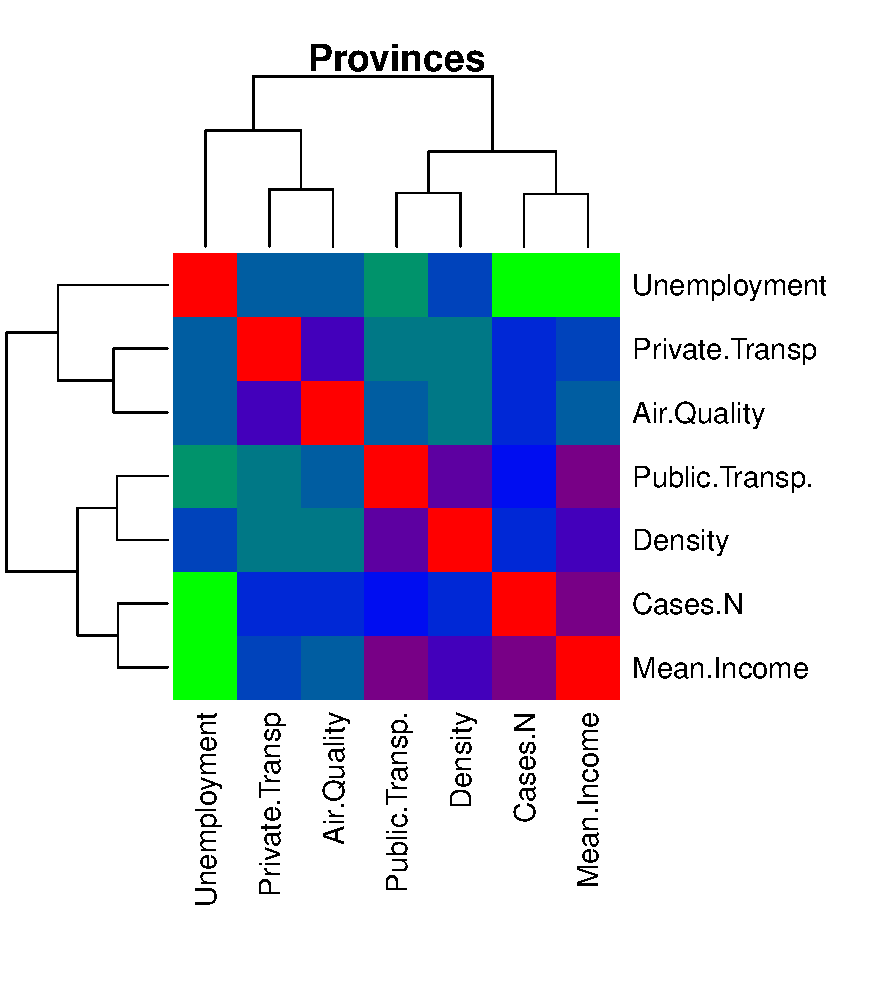
\includegraphics[scale=1]{Pic/Province_FULL_CorrMatrix.pdf}
\caption{The Correlation matrix for the Italian provinces accompanied by its heat-map as generated by the following dataset: local unemployment (2019), local private transport (2012 number of cars for 1000 residents), the air quality (2012) ,the local public transport (2012 measured as the demand for resident), the density  (2019 measured as resident for Km$^{2}$, the cumulative cases up to 26/08/2020 and the mean income (2019 measured in kEUR). Note that the public transport, the denisty the cumulative cases and the mean income are highly correlated. On the other hand the unemployment is negatively correlated to this first cluster}
\label{Province_corr_matrix}
\end{center}
\end{figure}

\begin{figure}[h]
\begin{center}
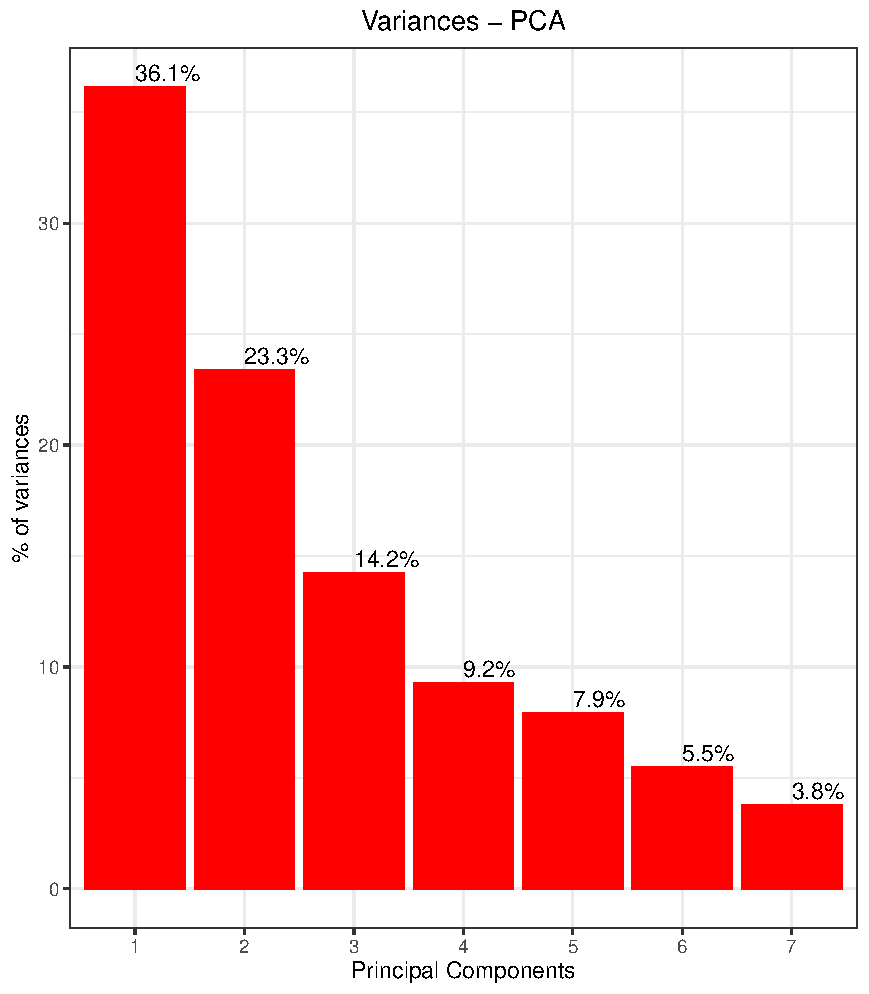
\includegraphics[scale=1]{Pic/Province_FULL_Variances.pdf}
\caption{Percentage of variance for each component of the dataset concerning the provinces. Note that using the first two, almost the 60 $\% $ of variance is captured, as consequence the information lost is almost the 40 $\%$ }
\label{Province_FULL_Variances}
\end{center}
\end{figure}

\begin{figure}[h]
\begin{center}
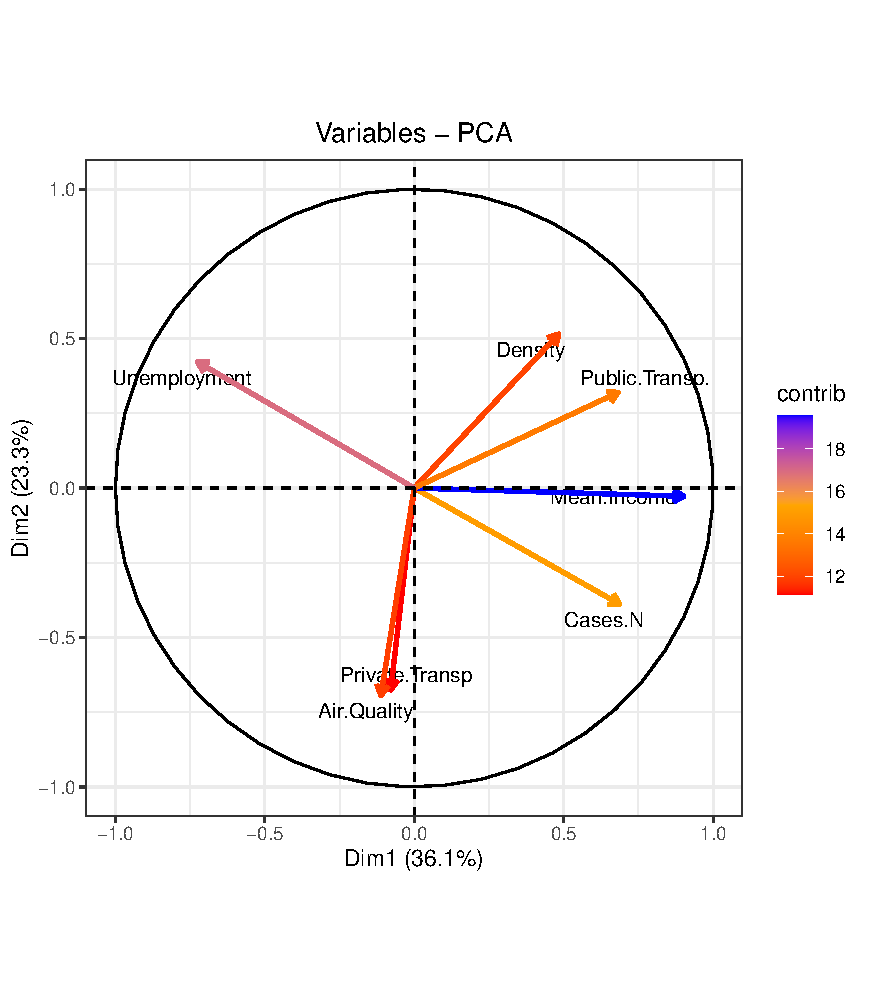
\includegraphics[scale=1]{Pic/Province_FULL_Variables-PCA.pdf}
\caption{2D plot of the loading vector for the dataset of provinces normalized on the unitary circle. The features, the date of their collection and unit of measure are the same of Fig. \ref{Province_FULL_Variables-PCA}}
\label{Province_FULL_Variables-PCA}
\end{center}
\end{figure}

\begin{figure}[h]
\begin{center}
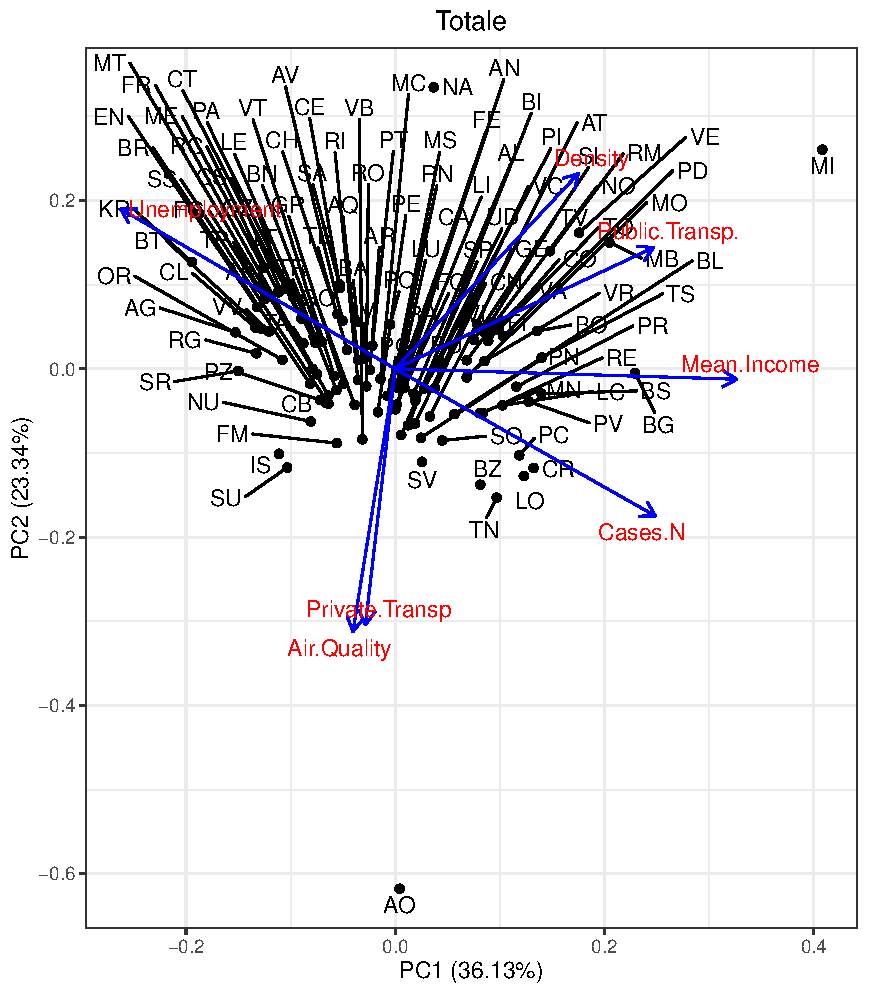
\includegraphics[scale=1]{Pic/Provinces_PCA_FULL.pdf}
\caption{The dataset of provinces plotted on the two principal components that capture the 60 $\% $ of variance. The provinces are labelled with their vehicle registration abbreviation. The features, the date of their collection and unit of measure are the same of Fig. \ref{Province_corr_matrix} }
\label{Provinces_PCA_FULL}
\end{center}
\end{figure}

\clearpage

\subsection{Regions}

Looking to the Fig. \ref{Regions_CorrMatrix},\ref{Regioni_PCA_loadings} and \ref{Regions_FULL_PCA} we found a positive correlation between the Mean Income and the Cases, as for the provinces,. This relation has the same explanation that was found in the previous paragraph. Furthermore here, since the overall number of tests are available as well as the number of deaths for COVID19, we see that these two normalized quantities are positively correlated with the cases. The causal connection for these three quantities is simple: in order to validate that a patient is infected a test is required, and a part of the infected patient are going to die for COVID19. The correlation matrix also highlights that there is a positive correlation between the number of people for general practitioner and the number of cases; moreover a higher number of normalized visit is negatively correlated with the number of cases and the mortality. The causal reason for this statistical correlation is currently under discussion but an interesting perspective, at a journalistic level, was performed on a Italian newspaper \cite{24plus}: the idea of the author is that the general practitioners play the role of sensor/sentinel for the COVID19 cases; as long as their number and their presence in all the cities is reduced, the health service is less sensitive to find new cases and the diffusion of the virus is favoured.  On the other side the quality index LEA,the normalized number of medical and the number of Public Structure Normalized  guards seems to play a weaker role. Finally it is worth nothing that, as shown in Fig. \ref{Region_variances} in the 2D plots \ref{Regioni_PCA_loadings} and \ref{Regions_FULL_PCA} only the 26.7 $ \% $ of information is lost.



\begin{figure}[h]
\begin{center}
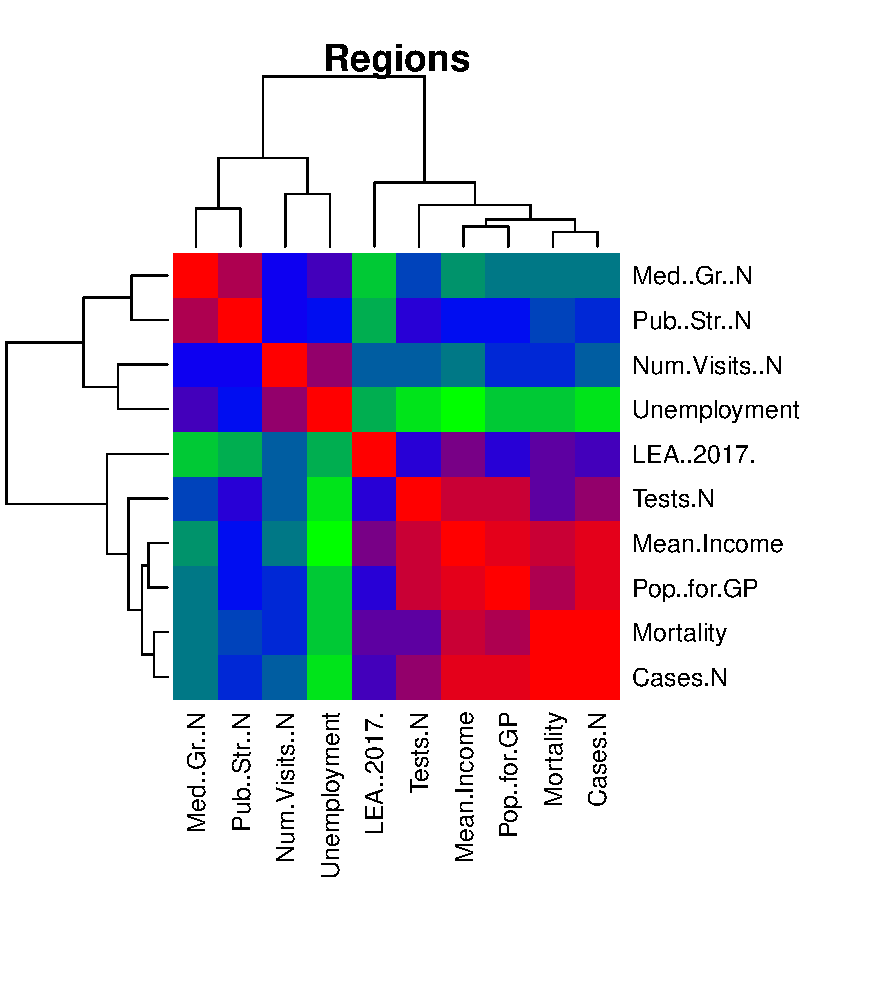
\includegraphics[scale=1]{Pic/Regions_CorrMatrix.pdf}
\caption{The Correlation matrix for the Italian regions accompanied by its heat-map as generated by the following dataset: the normalized number of medical guards (2017), the normalized number of structures for hospitalization (2017), the normalized number of visit for medical guards (2017), the unemployment ratio (2019), the essential assistance levels (LEA - 2017, the number of normalized tests (24/08/2020), the mean income (2019), the population for general practitioner  (2017), the normalized deaths for COVID19 (24/08/2020), and the normalized number of cases (24/08/2020) }
\label{Regions_CorrMatrix}
\end{center}
\end{figure}


\begin{figure}[h]
\begin{center}
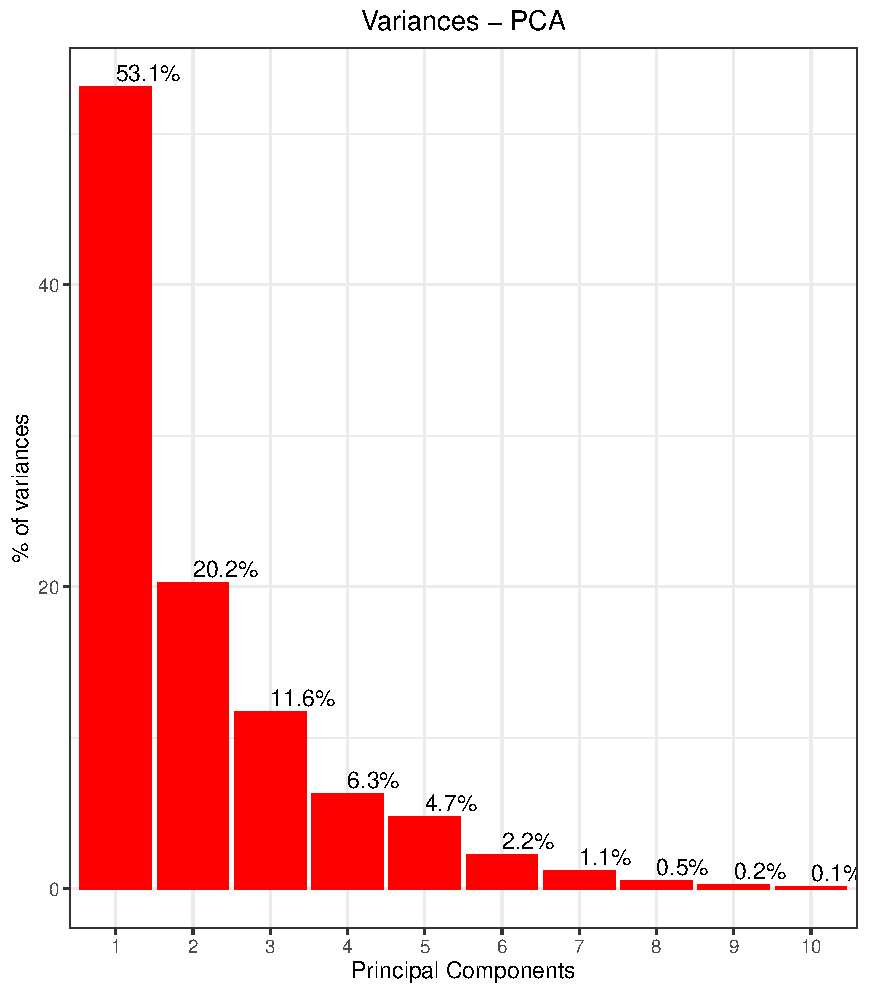
\includegraphics[scale=1]{Pic/Region_variances.pdf}
\caption{Percentage of variance for each component of the dataset concerning the provinces. Note that using the first two, the 73.3 $\% $ of variance is captured, as consequence the information lost is almost the 26.7 $\%$}
\label{Region_variances}
\end{center}
\end{figure}


\begin{figure}[h]
\begin{center}
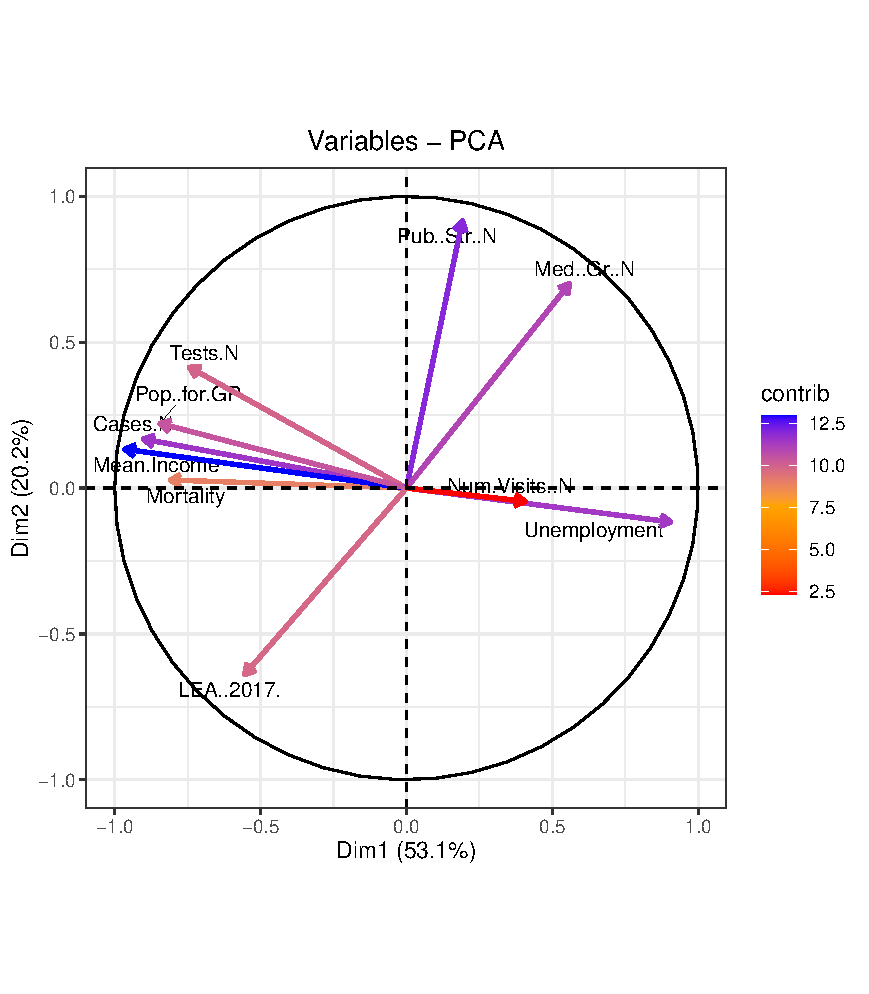
\includegraphics[scale=1]{Pic/Regioni_PCA_loadings.pdf}
\caption{2D plot of the loading vector for the dataset of regions normalized on the unitary circle. The features, the date of their collection and unit of measure are the same of Fig. \ref{Regions_CorrMatrix}}
\label{Regioni_PCA_loadings}
\end{center}
\end{figure}


\begin{figure}[h]
\begin{center}
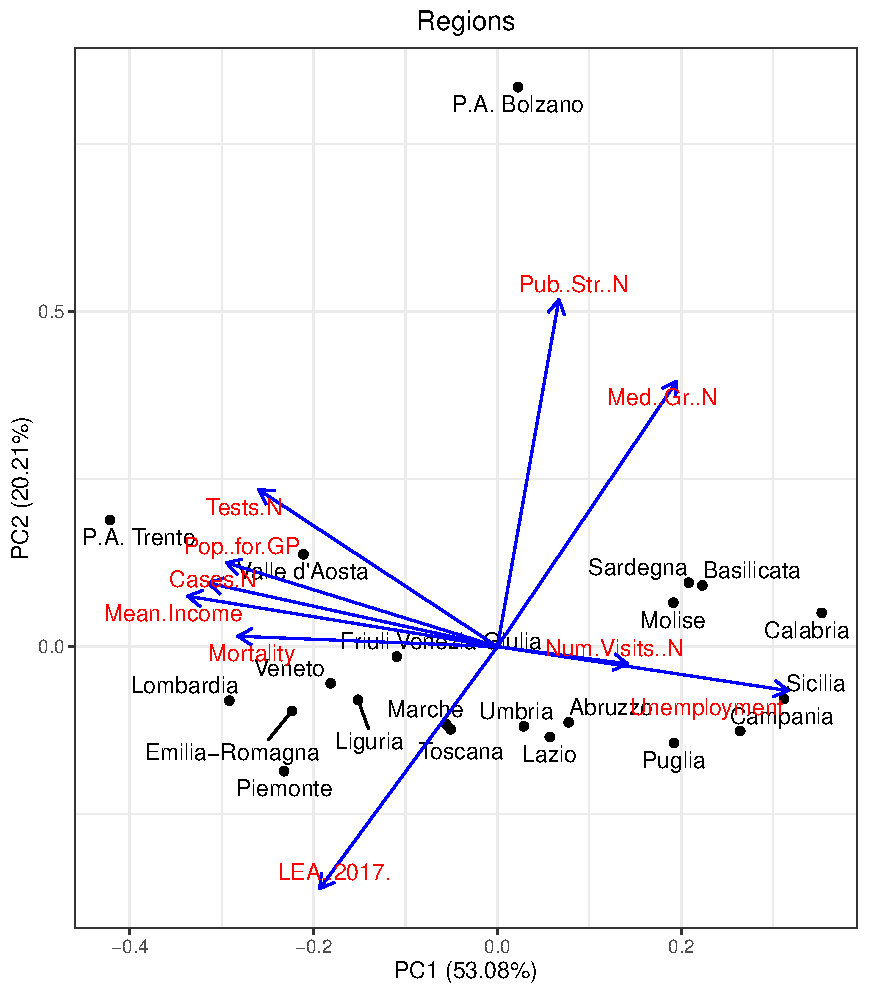
\includegraphics[scale=1]{Pic/Regions_FULL_PCA.pdf}
\caption{The dataset of regions plotted on the two principal components that capture the 73.3 $\% $ of variance. The features, the date of their collection and unit of measure are the same of Fig. \ref{Province_corr_matrix}}
\label{Regions_FULL_PCA}
\end{center}
\end{figure}


\clearpage

\subsection{Countries}

\begin{figure}[h]
\begin{center}
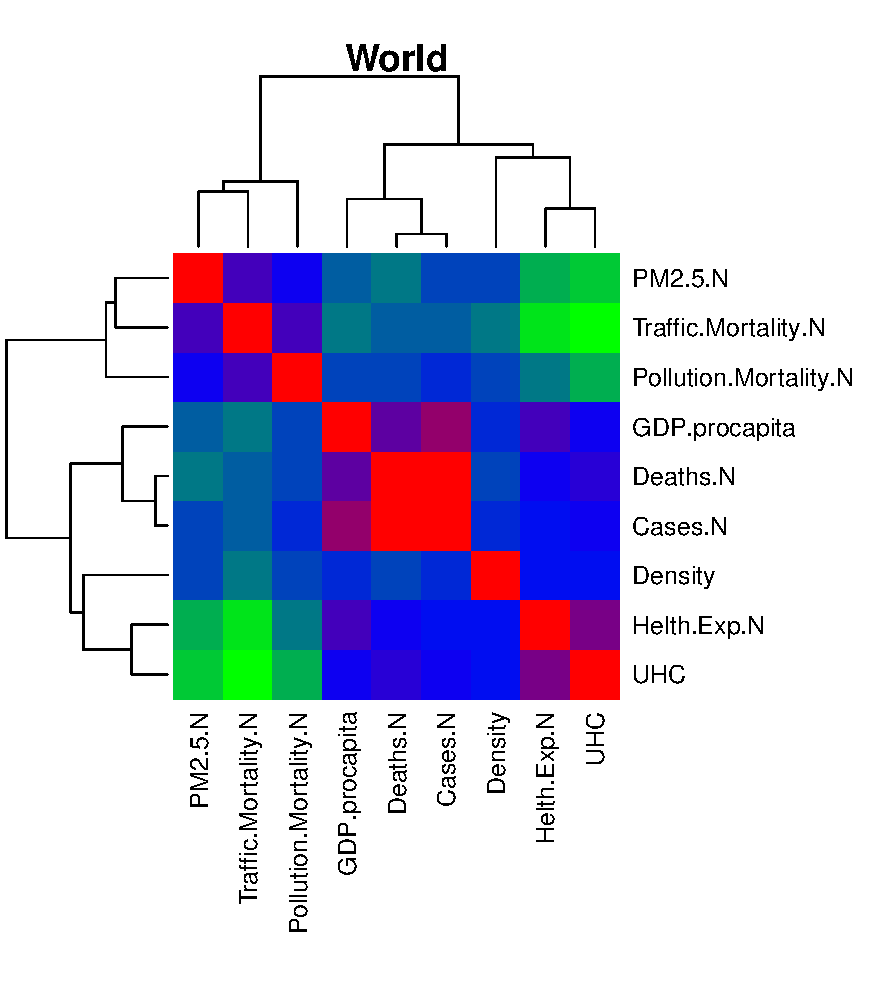
\includegraphics[scale=1]{Pic/CorrMatrix_WORLD.pdf}
\caption{The Correlation matrix for the a set of countries accompanied by its heat-map as generated by the following dataset:  }
\label{World_CorrMatrix}
\end{center}
\end{figure}


\begin{figure}[h]
\begin{center}
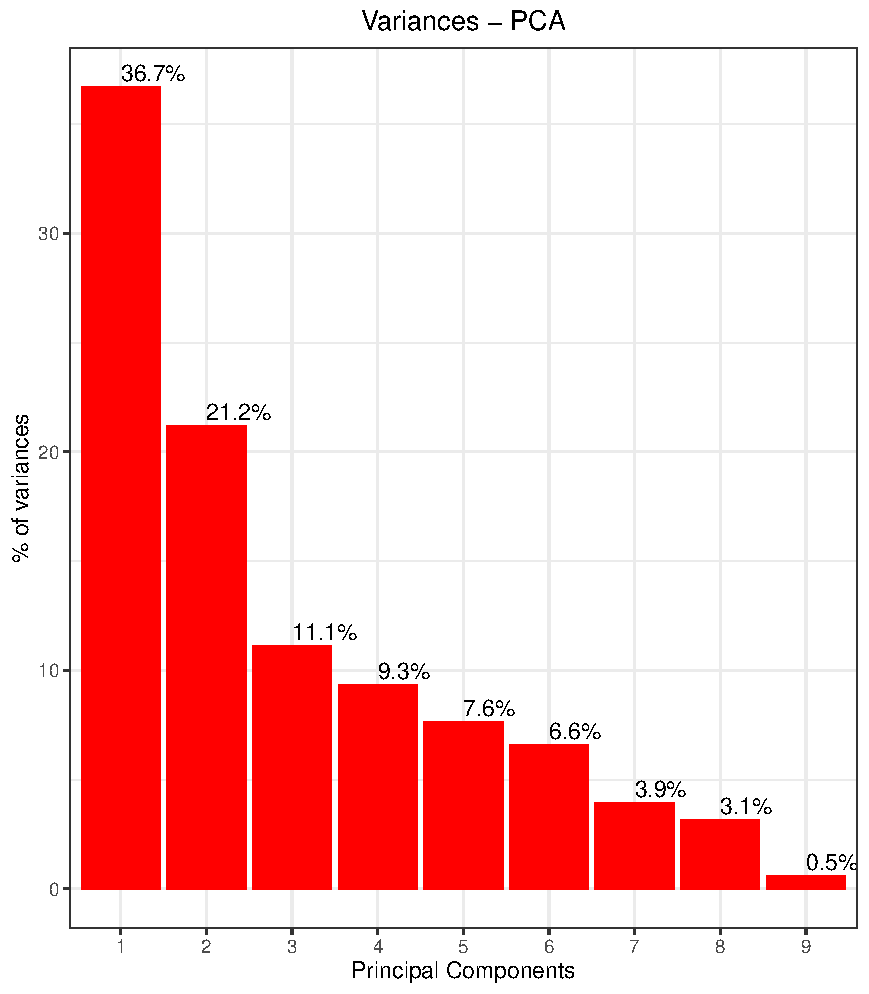
\includegraphics[scale=1]{Pic/Variances-PCA_WORLD.pdf}
\caption{Percentage of variance for each component of the dataset concerning the selected countries. Note that using the first two, the 57.9 $\% $ of variance is captured, as consequence the information lost is 42.1 $\%$}
\label{World_variances}
\end{center}
\end{figure}


\begin{figure}[h]
\begin{center}
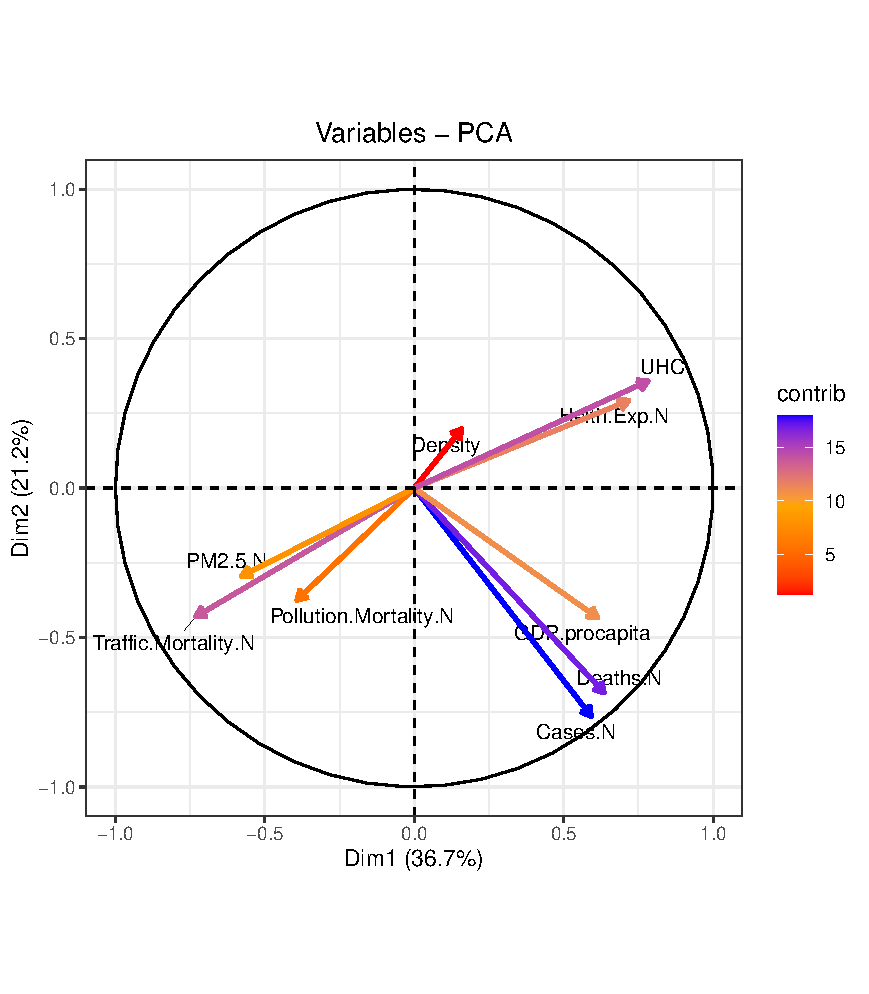
\includegraphics[scale=1]{Pic/PCA-Loadings_WORLD.pdf}
\caption{2D plot of the loading vector for the dataset of the selected countries normalized on the unitary circle. The features, the date of their collection and unit of measure are the same of Fig. \ref{World_CorrMatrix}}
\label{World_PCA_loadings}
\end{center}
\end{figure}


\begin{figure}[h]
\begin{center}
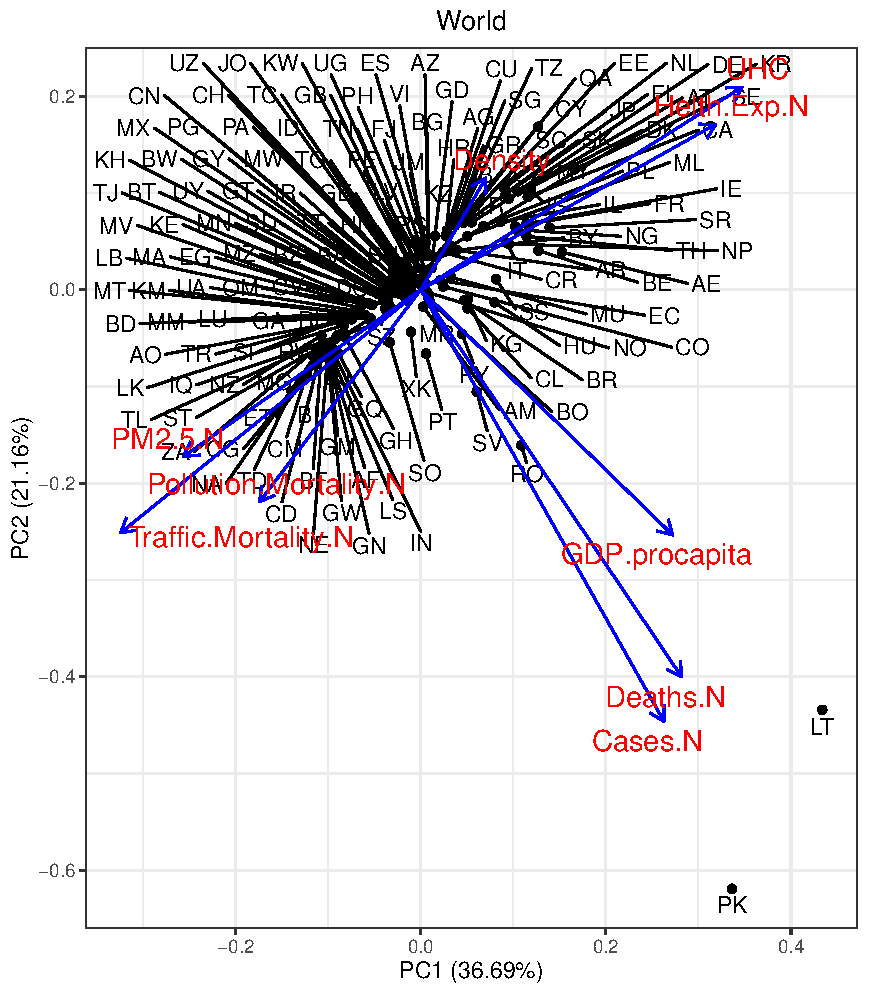
\includegraphics[scale=1]{Pic/World_FULLPCA.pdf}
\caption{The dataset of countries plotted on the two principal components that capture the 57.9 $\% $ of variance. The features, the date of their collection and unit of measure are the same of Fig. \ref{World_CorrMatrix}}
\label{World_FULL_PCA}
\end{center}
\end{figure}




\clearpage



%------------------------------------------------



%----------------------------------------------------------------------------------------
%	BIBLIOGRAPHY
%----------------------------------------------------------------------------------------

\renewcommand{\refname}{\spacedlowsmallcaps{References}} % For modifying the bibliography heading

\bibliographystyle{unsrt}

\bibliography{bibliography.bib} % The file containing the bibliography

%----------------------------------------------------------------------------------------

\end{document}